\chapter{Fuerzas, quarks y los primeros multipletes de hadrones}

\section{Partículas, campos y el tercer elemento que falta}

Las ondas son configuraciones de campos, así que, en esta discusión, ambas descripciones están estrechamente relacionadas. La mecánica cuántica establece que la energía de una onda de este tipo viene en unidades discretas e indivisibles. Esas unidades son sus cuantos, y llamamos partículas a los cuantos de un campo. Con esta relación en mente, ya hemos hablado de ecuaciones de onda, principios de acción y las propiedades generales que portan las partículas: energía, momento, espín y la distinción entre bosones--fermiones. Los fermiones se resisten a ocupar el mismo estado; los bosones pueden congregarse y condensarse en un solo estado.

Un lagrangiano cuántico también registra las interacciones. Los productos de campos representan vértices en los que entran y salen partículas. Por ejemplo, un término con cuatro potencias de un campo representa un vértice de interacción de cuatro patas. Así, el principio de acción se convierte en un inventario compacto de los procesos posibles entre partículas.

La siguiente tarea es nombrar las partículas---no exactamente una por una, sino por familias---y dar a cada una cierta personalidad: sus propiedades, sus interacciones y su lugar en la física ordinaria. Sin embargo, antes de hacer esa lista, aún falta un lado del triángulo conceptual:
\begin{itemize}
\item partículas,
\item campos de los que esas partículas son cuantos,
\item fuerzas asociadas a procesos de intercambio que involucran esos mismos cuantos.
\end{itemize}

La palabra \emph{elemental} debe seguir siendo provisional. Toda definición plausible de partícula elemental, en contraposición a compuesta, acaba por toparse con un caso escurridizo, y volveremos sobre ese problema. Por ahora, supongamos que existen campos fundamentales y llamemos partículas elementales a sus cuantos. Si un campo eléctrico da lugar a fuerzas eléctricas y un campo gravitatorio a fuerzas gravitatorias, el campo del electrón también debe participar en fuerzas. El triángulo solo puede cerrarse si la fuerza tiene una descripción en términos de partículas además de una descripción en términos de campos.

Por tanto, deduciremos la lógica de la fuerza de dos maneras. Primero recurriremos a la energía clásica de campo; después preguntaremos cómo se manifiesta la misma interacción cuando se resuelve un campo en sus cuantos. Solo una vez establecido ese puente comenzaremos el catálogo de partículas.

\section{La fuerza a partir de la energía de campo en la electrodinámica clásica}

Coloquemos dos cargas en el espacio. Una manera de hallar la fuerza entre ellas es citar la ley del inverso del cuadrado. Una manera más reveladora es preguntarnos qué hacen las cargas al espacio: crean campos eléctricos, y esos campos almacenan energía.

Conviene separar cada carga de la forma espacial de su campo,
\begin{equation}
\mathbf E_i=q_i\widehat{\mathbf E}_i,
\end{equation}
aunque nada depende de conservar la notación con sombrero. Con ambas cargas presentes, la linealidad da
\begin{equation}
\mathbf{E}=\mathbf{E}_1+\mathbf{E}_2.
\end{equation}
Salvo por la elección de unidades, la energía electrostática del campo tiene la forma
\begin{equation}
U_{\text{field}}\propto\int d^3x\,\mathbf{E}^2.
\end{equation}
Al sustituir la suma de los dos campos se obtiene
\begin{align}
U_{\text{field}}
&\propto\int d^3x\,(\mathbf{E}_1+\mathbf{E}_2)^2 \\
&\propto\int d^3x\,\bigl(\mathbf{E}_1^2+\mathbf{E}_2^2
  +2\mathbf{E}_1\!\cdot\!\mathbf{E}_2\bigr).
\end{align}

Los dos primeros términos son autoenergías. Trasladar cualquiera de las cargas desplaza su campo junto con ella y no cambia la integral correspondiente. Esa energía contribuye, a través de \(E=mc^2\), a la masa medida de la partícula cargada aislada. La manera en que esta autoenergía se incorpora a la masa medida corresponde al tema posterior de la renormalización. Ninguna de estas energías, que no dependen de la posición, contribuye a la fuerza entre las dos partículas.

El término cruzado es distinto. No pertenece por separado a ninguna de las partículas y solo existe cuando están presentes ambos campos. Si se separan las cargas a una distancia muy grande, las regiones donde sus campos son apreciables apenas se solapan. Al acercarse las cargas, cambia el solapamiento. Por tanto, la energía de interacción, que depende de la configuración, es proporcional a
\begin{equation}
U_{\text{int}}(r)\propto q_1q_2\int d^3x\,
\widehat{\mathbf E}_1\!\cdot\!\widehat{\mathbf E}_2.
\end{equation}
Para dos cargas puntuales separadas por \(r\), al evaluar la integral se obtiene la conocida dependencia
\begin{equation}
U_{\text{int}}(r)\propto\frac{q_1q_2}{r}.
\end{equation}
La fuerza radial es su gradiente negativo,
\begin{equation}
\mathbf F_{12}=-\boldsymbol\nabla_{\mathbf r}U_{\text{int}},
\qquad
|\mathbf F_{12}|\propto\frac{|q_1q_2|}{r^2}.
\end{equation}
\editorialnote{El argumento oral identifica el término cruzado con la fuerza de Coulomb del inverso del cuadrado sin detenerse en el potencial. Aquí se escribe explícitamente el término intermedio estándar \(U_{\mathrm{int}}\propto1/r\) para que su gradiente dé la fuerza \(1/r^2\) indicada.}

La ley de fuerza se ha convertido en la derivada de la parte de la energía del campo que depende de la posición relativa. A gran distancia, los dos objetos son efectivamente independientes. Al acercarlos, el campo entre ellos se reorganiza; el cambio resultante de energía es la interacción.

Pero si un campo puede resolverse en cuantos, la historia no puede acabar aquí. La misma fuerza debe tener una explicación en términos de partículas.

\section{Intercambio molecular: dos protones y un electrón}

Antes de volver a la electrodinámica, consideremos un sistema en el que el intercambio resulta más fácil de visualizar: dos protones y un electrón. El intercambio es solo uno de varios orígenes de las fuerzas moleculares, pero este ejemplo permite ver la relación entre intercambio, energía y fuerza. No se ofrece como sustituto de la electrodinámica cuántica.

Si hay un protón y el otro está infinitamente lejos, el electrón puede ocupar el estado fundamental hidrogenoide centrado en el primer protón. Su función de onda está localizada cerca de ese centro de fuerza.

\begin{figure}[h]
\centering
\includegraphics[width=0.72\textwidth]{lecture_01_figure_02.png}

\medskip

\begin{tikzpicture}[scale=0.95]
\draw (-0.2,0) -- (6.4,0);
\fill (1.3,0) circle (2pt);
\draw[smooth] plot coordinates {(0.1,0.15) (0.8,1.15) (1.5,1.75) (2.2,1.1) (3.0,0.35) (3.8,0.12)};
\node at (1.3,-0.35) {$p$};
\node at (2.7,1.55) {$\psi_1(x)$};
\end{tikzpicture}
\caption{Una función de onda del estado fundamental hidrogenoide localizada cerca de un protón.}
\lectureframe{00:14:32}
\end{figure}
\editorialnote{La etiqueta \(\psi_1(x)\) en el redibujo nombra el perfil localizado descrito en 00:14:30--00:14:32; no se ha copiado de una etiqueta legible en la pizarra.}

Coloquemos ahora un segundo protón a una distancia grande, pero finita. Por simetría, existe un segundo estado localizado con la misma energía de centro único, esta vez centrado en el protón de la derecha.

\begin{figure}[h]
\centering
\includegraphics[width=0.78\textwidth]{lecture_01_figure_03.png}

\medskip

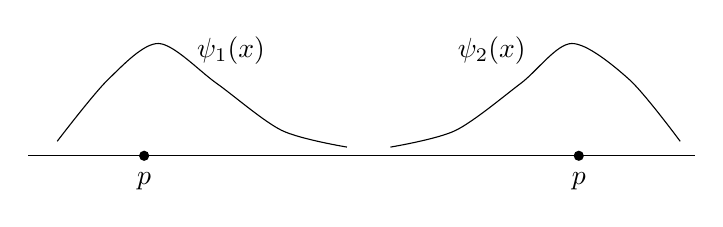
\begin{tikzpicture}[scale=0.92]
\draw (-0.2,0) -- (9.0,0);
\fill (1.4,0) circle (2pt);
\fill (7.4,0) circle (2pt);
\draw[smooth] plot coordinates {(0.2,0.2) (0.9,1.05) (1.6,1.55) (2.4,1.0) (3.3,0.35) (4.2,0.12)};
\draw[smooth] plot coordinates {(4.8,0.12) (5.7,0.35) (6.6,1.0) (7.3,1.55) (8.1,1.05) (8.8,0.2)};
\node at (1.4,-0.35) {$p$};
\node at (7.4,-0.35) {$p$};
\node at (2.6,1.45) {$\psi_1(x)$};
\node at (6.2,1.45) {$\psi_2(x)$};
\end{tikzpicture}
\caption{Los dos perfiles localizados que se usan para formar la superposición de equilibrio cuando se permite el túnel.}
\lectureframe{00:17:54}
\end{figure}
\editorialnote{Las etiquetas \(\psi_1(x)\) y \(\psi_2(x)\) identifican los dos perfiles comentados en 00:17:41--00:17:56; los símbolos son etiquetas esquemáticas añadidas para facilitar la lectura.}

A separación infinita, los dos estados son degenerados: localizar el electrón a la izquierda o a la derecha cuesta la misma energía. A separación finita, se hace posible un proceso nuevo. El electrón puede atravesar por efecto túnel la región clásicamente prohibida y pasar de un centro al otro. Observar una trayectoria a través de la barrera perturbaría el estado; ``el salto'' describe la evolución cuántica, no una película de un recorrido clásico.

En equilibrio, la probabilidad de encontrar el electrón cerca de cualquiera de los protones es la misma. Por tanto, la normalización aporta el factor \(1/\sqrt2\), y el estado de equilibrio de menor energía es, aproximadamente,
\begin{equation}
\psi_+(x)\approx \frac{\psi_1(x)+\psi_2(x)}{\sqrt2}.
\end{equation}

El signo de aproximación es importante. La verdadera función de onda de dos centros no es exactamente la suma de dos orbitales hidrogenoides inalterados; se ajusta en la región de solapamiento. Lo que necesitamos aquí es que el estado simétrico de equilibrio queda por debajo de la energía de centro único aislado. En el lenguaje del hamiltoniano, las configuraciones izquierda y derecha están acopladas por un elemento de matriz no diagonal. Al permitir que el electrón ocupe su superposición coherente, la energía disminuye.

\section{De la energía reducida a una fuerza efectiva}

A grandes separaciones entre los protones, la contribución inducida por el electrón \(E_e(r)\) tiende al valor correspondiente a los átomos separados. A separaciones menores, el túnel y la superposición la reducen. El potencial completo de dos protones--y un electrón también debe incluir la repulsión directa entre protones,
\begin{equation}
V_{\mathrm{tot}}(r)=V_{pp}(r)+E_e(r).
\end{equation}

Esto vuelve a conectar el ejemplo molecular con el argumento basado en la energía de campo. Los esquemas de funciones de onda y la curva cualitativa de \(E_e(r)\) son dos formas de ver el mismo cálculo; el equilibrio lo determina la suma \(V_{\mathrm{tot}}(r)\).

\begin{figure}[h]
\centering
\includegraphics[width=0.78\textwidth]{lecture_01_figure_04.png}

\medskip

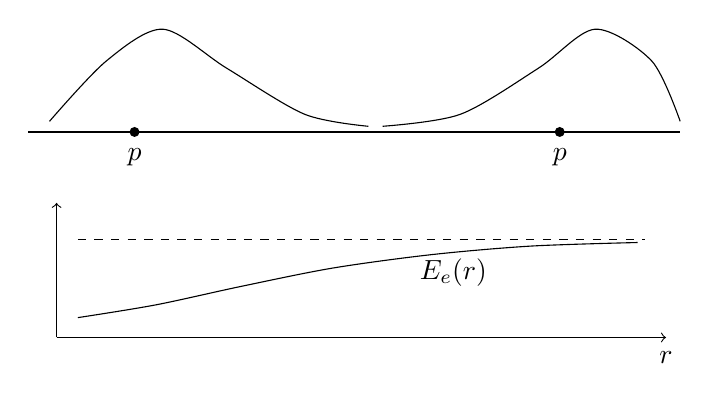
\begin{tikzpicture}[scale=0.9]
\draw (-0.2,3.0) -- (9.0,3.0);
\fill (1.3,3.0) circle (2pt);
\fill (7.3,3.0) circle (2pt);
\draw[smooth] plot coordinates {(0.1,3.15) (0.9,4.0) (1.7,4.45) (2.6,3.9) (3.7,3.25) (4.6,3.08)};
\draw[smooth] plot coordinates {(4.8,3.08) (5.9,3.25) (7.0,3.9) (7.8,4.45) (8.6,4.0) (9.0,3.15)};
\node at (1.3,2.65) {$p$};
\node at (7.3,2.65) {$p$};

\draw[->] (0.2,0.1) -- (0.2,2.0);
\draw[->] (0.2,0.1) -- (8.8,0.1);
\draw[dashed] (0.5,1.48) -- (8.5,1.48);
\draw[smooth] plot coordinates {(0.5,0.38) (1.6,0.56) (2.8,0.82) (4.1,1.08) (5.5,1.27) (6.9,1.39) (8.4,1.44)};
\node at (5.8,1.02) {$E_e(r)$};
\node at (8.8,-0.18) {$r$};
\end{tikzpicture}
\caption{Solapamiento de las funciones de onda arriba y energía inducida por el electrón abajo. Esta última tiende a la asíntota de los átomos separados a medida que aumenta \(r\); el potencial total entre protones también debe incluir su repulsión de Coulomb.}
\lectureframe{00:20:28}
\end{figure}
\editorialnote{Las etiquetas \(E_e(r)\) y \(r\) identifican la curva de energía y la separación comentadas en 00:19:12--00:20:38; el fragmento conservado de la pizarra no permite leer esas etiquetas de los ejes.}

Las dos fuerzas correspondientes se obtienen de los gradientes de la energía,
\begin{equation}
F_{e}(r)=-\frac{dE_e}{dr},
\qquad
F_{\mathrm{tot}}(r)=-\frac{dV_{\mathrm{tot}}}{dr}.
\end{equation}
Por tanto, el sistema tiende hacia una energía total menor. Allí donde \(E_e(r)\) disminuye al acercarse los protones, el intercambio aporta una contribución atractiva; que exista o no una separación de equilibrio depende de su competencia con \(V_{pp}(r)\). Este es el mecanismo elemental que subyace a un enlace covalente: el electrón se comparte porque el estado compartido es energéticamente favorable.

En el cálculo clásico, el solapamiento de los campos eléctricos cambia la energía. Aquí, dos centros de fuerza permiten un estado cuántico de menor energía. Ambos mecanismos producen una fuerza porque la energía de equilibrio depende de la configuración.

El lenguaje del intercambio puede resumirse mediante un esquema de líneas de mundo. No debe interpretarse como una trayectoria observada; representa amplitudes para que el electrón esté asociado con cualquiera de los protones.

\begin{figure}[h]
\centering
\begin{tikzpicture}[scale=1.0]
\draw (0,0) -- (0,4.4);
\draw (4.8,0) -- (4.8,4.4);
\draw (0,0.9) .. controls (1.6,1.7) and (3.2,1.7) .. (4.8,2.5);
\draw (4.8,2.9) .. controls (3.2,2.1) and (1.6,2.1) .. (0,3.9);
\node at (0,-0.35) {$p$};
\node at (4.8,-0.35) {$p$};
\node at (2.35,1.55) {$e^-$};
\node at (2.35,2.55) {$e^-$};
\end{tikzpicture}
\caption{Intercambio del electrón entre las líneas de mundo de dos protones, entendido como un esquema de amplitudes cuánticas y no como una trayectoria observada.}
\end{figure}

\begin{classroomqa}
\audiencequestion{¿Puede entenderse la atracción simplemente como un apantallamiento del protón por el electrón o como una reducción de su carga?\lecturetimestamp{00:23:26}}
\lecturerresponse{No. La reducción de la carga no es la interpretación correcta de este efecto. Lo esencial es que, al sumar las dos funciones de onda localizadas, se obtiene un estado cuya energía es ligeramente menor que la de cada estado localizado por separado.}
\end{classroomqa}

\begin{classroomqa}
\audiencequestion{¿Es esto lo que quería decir Feynman al afirmar que a la ``luz le gusta la luz''?\lecturetimestamp{00:23:51}}
\lecturerresponse{No. Lo más probable es que esa frase se refiera a la estadística de Bose: los fotones favorecen los estados comunes, mientras que los electrones obedecen el principio de exclusión. El efecto molecular que tratamos aquí es el túnel entre dos centros.}
\end{classroomqa}

Los dos protones siguen repeliéndose electrostáticamente. El intercambio tiene menor alcance que la interacción de Coulomb, así que hay que considerar el potencial total y no cada contribución por separado. Sin embargo, a ciertas separaciones el ion molecular \(\mathrm H_2^+\) está ligado; en un sistema neutro de dos electrones, la repulsión de carga a largo alcance está ausente y el enlace covalente resulta aún más familiar.

\begin{classroomqa}
\audiencequestion{¿Colocar el electrón entre los protones reduce principalmente su repulsión electrostática?\lecturetimestamp{00:24:33}}
\lecturerresponse{Reduce un poco la repulsión, pero ese no es el efecto principal. La fuerza debida al intercambio electrónico tiene menor alcance que la repulsión de Coulomb. Se aprecia con mayor claridad en un sistema neutro de dos electrones, donde no existe una fuerza electrostática de largo alcance entre los átomos, pero el túnel sigue produciendo una atracción.}
\end{classroomqa}

\begin{classroomqa}
\audiencequestion{¿Está realmente ligado el ion molecular con carga positiva \(\mathrm H_2^+\), que tiene un solo electrón?\lecturetimestamp{00:26:06}}
\lecturerresponse{Sí. A una separación suficientemente pequeña, la atracción por intercambio basta para superar la repulsión de Coulomb entre protones--.}
\end{classroomqa}

\begin{classroomqa}
\audiencequestion{¿La configuración de dos centros crea una tercera fuerza?\lecturetimestamp{00:26:24}}
\lecturerresponse{No se introduce ninguna fuerza fundamental nueva. La ecuación de Schr\"odinger en el potencial combinado de los dos protones tiene una energía de equilibrio distinta de la del problema de un solo centro; la derivada de ese cambio de energía es la fuerza efectiva.}
\end{classroomqa}

\begin{classroomqa}
\audiencequestion{¿Es la reducción de energía un ejemplo de entrelazamiento cuántico?\lecturetimestamp{00:27:06}}
\lecturerresponse{No en el sentido habitual de dos partículas: solo hace falta un electrón. La característica matemática pertinente es un elemento de matriz no diagonal del hamiltoniano que acopla los estados de la izquierda y de la derecha.}
\end{classroomqa}

\begin{classroomqa}
\audiencequestion{¿Qué ocurre con el intercambio a alta temperatura?\lecturetimestamp{00:27:37}}
\lecturerresponse{A temperaturas extremas, el electrón se ioniza y deja atrás la molécula por completo. A una energía de excitación menor, puede ocupar un orbital más grande, lo que cambia el solapamiento y, por consiguiente, la fuerza. Se trata de una corrección dependiente del estado, no de un mecanismo general nuevo.}
\end{classroomqa}

\section{Intercambio de fotones y las primeras entradas de la tabla}

¿Puede describirse la fuerza de Coulomb con el mismo lenguaje del intercambio? Una partícula cargada interactúa con el campo electromagnético, cuyos cuantos son fotones. Clásicamente, resolvemos el campo eléctrico alrededor de la carga. En teoría cuántica de campos, describimos esa interacción mediante emisión y absorción de fotones.

Una partícula cargada física no es simplemente una carga desnuda. Su estado es una superposición cuántica que contiene una componente de electrón desnudo, un electrón con un fotón, un electrón con dos fotones, y así sucesivamente. En una notación deliberadamente esquemática,
\begin{equation}
\begin{aligned}
\ket{e_{\mathrm{phys}}}
={}&a_0\ket e
+a_1\ket{e+\text{one photon}}
\\
&+a_2\ket{e+\text{two photons}}+\cdots .
\end{aligned}
\end{equation}
Esta notación solo registra la jerarquía de componentes con distinto número de fotones; no especifica los momentos de los fotones ni pretende construir por completo un estado cargado interactuante.
Los fotones que rodean al electrón se emiten y se reabsorben, en lugar de escapar como radiación libre. Sus efectos pueden medirse, aunque no se detectan de la misma manera que los fotones que se propagan libremente. Si se coloca una segunda carga cerca, un fotón emitido por una carga puede ser absorbido por la otra. Entonces, la energía de los dos estados vestidos deja de ser igual a la simple suma de las energías de dos estados aislados.

La analogía de clase es la de dos malabaristas, cada uno haciendo malabares con un conjunto de pelotas. Cuando están lejos, cada cual hace malabares por su cuenta. Si se acercan lo suficiente, uno puede atrapar una pelota que el otro le haya lanzado. En el lenguaje de los diagramas de Feynman, ese objeto compartido es el fotón intercambiado. La analogía no representa una trayectoria microscópica, pero muestra por qué la proximidad permite un proceso nuevo.

Ahora contamos con dos descripciones que van más allá de memorizar la ley de Coulomb. La teoría clásica de campos suma los campos y eleva al cuadrado el resultado. La teoría cuántica de campos suma amplitudes en las que se intercambian cuantos. En este sentido, existe una correspondencia uno a uno entre partículas, campos y fuerzas. Los electrones median el intercambio molecular, los fotones median el intercambio electromagnético y cualquier partícula que pueda intercambiarse puede contribuir a una fuerza en el contexto adecuado. Así, la afirmación conocida de que la naturaleza tiene cuatro interacciones fundamentales es una clasificación de nivel más general; en el lenguaje del intercambio, cada especie intercambiable puede generar su propia contribución efectiva a una fuerza.

Por fin ha llegado el momento de nombrar las partículas, enumerar sus propiedades e indicar en qué procesos pueden intervenir. Escribir de una vez todo el modelo estándar solo daría lugar a una larga prueba de memoria, así que dividiremos las partículas en grupos pequeños, cuyos integrantes guardan relaciones sencillas, y veremos qué puede hacer cada grupo.

El catálogo completo es engorroso porque no entendemos por qué existen precisamente estas partículas y no otras partículas imaginables. La consistencia matemática impone algunas relaciones: una vez que existen varios integrantes de un patrón, puede ser necesario que exista otro para completarlo. Esas relaciones reducen el número de hechos independientes, pero solo en una medida modesta. Siguen sin explicarse muchos tipos de partículas y muchos parámetros. Entender esa estructura aún incompleta es necesario para comprender qué buscan descubrir los experimentos posteriores.

\begin{figure}[h]
\centering
\includegraphics[width=0.7\textwidth]{lecture_01_figure_05.png}
\caption{La primera entrada de la tabla de partículas identifica el fotón mediante \(\gamma\) y su campo mediante el potencial vector \(A\).}
\lectureframe{00:39:11}
\end{figure}

La primera identificación campo--cuanto es
\begin{equation}
\gamma \leftrightarrow A.
\end{equation}
Aquí \(A\) es el potencial vector electromagnético. El fotón es un bosón de espín uno, con carga eléctrica nula, número bariónico nulo y masa en reposo nula. El campo del electrón se denota convencionalmente \(\psi_e\); sus partes de creación y aniquilación actúan sobre estados de electrón y positrón.

Nuestra tabla registra el nombre, el símbolo de la partícula, el campo, el tipo —bosón o fermión—, la carga eléctrica \(Q\), el número bariónico \(B\) y la masa:

\begin{table}[h]
\centering
\resizebox{\linewidth}{!}{%
\begin{tabular}{lllllll}
Nombre & Símbolo & Campo & Tipo & \(Q\) & \(B\) & Masa \\
Fotón & \(\gamma\) & \(A\) & bosón & \(0\) & \(0\) & \(0\) \\
Electrón & \(e^-\) & \(\psi_e\) & fermión & \(-1\) & \(0\) & \(0.51\,\mathrm{MeV}\) \\
Positrón & \(e^+\) & \(\psi_e\) & fermión & \(+1\) & \(0\) & \(0.51\,\mathrm{MeV}\)
\end{tabular}
}%
\caption{Las entradas del fotón, el electrón--y el positrón, que dan comienzo al catálogo de partículas.}
\end{table}

La relación entre electrón y positrón es mutua: cada uno es la antipartícula del otro. Llamar ``partícula'' al estado con carga negativa es una convención. Medimos la carga eléctrica en unidades del valor absoluto de la carga del electrón, de modo que
\begin{equation}
Q(e^-)=-1,\qquad Q(e^+)=+1.
\end{equation}
La masa se mide en unidades de energía usando \(E=mc^2\). Un electrón voltio es la energía que adquiere una carga \(e\) al atravesar una diferencia de potencial de un voltio,
\begin{equation}
1\,\mathrm{eV}=e\,(1\,\mathrm V).
\end{equation}
Esta unidad surge de forma natural en física atómica: como escala atómica aproximada, ionizar el hidrógeno requiere unos \(13.5\,\mathrm{eV}\). Las masas de las partículas requieren millones o miles de millones de electronvoltios. La masa del electrón es
\begin{equation}
m_e c^2 \approx 0.511\,\mathrm{MeV}.
\end{equation}

\begin{classroomqa}
\audiencequestion{¿La masa del electrón debería ser exactamente medio MeV?\lecturetimestamp{00:44:02}}
\lecturerresponse{No. El valor redondeado conveniente \(0.51\,\mathrm{MeV}\) no está fijado en exactamente medio por ningún principio; es un parámetro medido.}
\end{classroomqa}

El proceso elemental de la electrodinámica cuántica tiene una línea de fermión cargado que entra, otra que sale y una línea de fotón conectada. Reordenar las patas o cruzarlas permite que el mismo vértice describa la emisión o absorción de un fotón, o un proceso con positrones. En la notación esquemática no covariante que usamos aquí, la interacción contiene
\begin{equation}
\mathcal{L}_{\mathrm{int}}\sim e\,\psi_e^\dagger \psi_e A.
\end{equation}
Al desarrollar los campos en operadores de creación y aniquilación se obtienen términos que eliminan un electrón entrante, crean un electrón saliente y crean o aniquilan un fotón. El acoplamiento \(e\) aporta un factor en el vértice. Así, para la emisión de un fotón cuando un electrón se dispersa o se acelera,
\begin{equation}
\mathcal{A}_{\mathrm{vertex}}\propto e,
\qquad
P_{\mathrm{emission}}\propto e^2.
\end{equation}
El impacto de un electrón contra el blanco de un tubo de rayos X es una situación práctica en la que importa esta probabilidad de emisión de fotones. Las combinaciones reiteradas del mismo vértice generan los procesos de la electrodinámica cuántica, incluido el cambio de energía que se interpreta como la fuerza entre cargas.

Por tanto, resulta útil representar el vértice de forma esquemática.

\begin{figure}[h]
\centering
\begin{tikzpicture}[scale=1.0]
\fill (0,0) circle (1.5pt);
\draw (-1.6,-1.2) -- (0,0) -- (1.6,-1.2);
\draw (0,0) -- (0,1.8);
\node at (-1.8,-1.4) {$e^-$};
\node at (1.8,-1.4) {$e^-$};
\node at (0.35,1.95) {$\gamma$};
\end{tikzpicture}
\caption{Esquema topológico del vértice elemental de la electrodinámica cuántica: entra una línea de fermión cargado, sale otra y se conecta una línea de fotón. La pata recta del fotón es aquí solo una convención gráfica simplificada.}
\end{figure}

La contribución del intercambio a la fuerza conecta dos vértices de este tipo:

\begin{figure}[h]
\centering
\begin{tikzpicture}[scale=1.0]
\draw (0,0) -- (0,4.0);
\draw (4.8,0) -- (4.8,4.0);
\draw (0,2.0) -- (4.8,2.0);
\node at (0,-0.35) {$e^-$};
\node at (4.8,-0.35) {$e^-$};
\node at (2.4,2.3) {$\gamma$};
\end{tikzpicture}
\caption{Esquema topológico del intercambio de fotones, que proporciona la descripción de la interacción de Coulomb en teoría cuántica de campos.}
\end{figure}

Una vez cerrado el triángulo partícula--campo--fuerza, podemos continuar con el catálogo.

\section{Quarks, número bariónico y el enigma de las familias}

Si este catálogo se hubiera escrito hacia 1960, probablemente los protones y neutrones habrían seguido a los electrones y fotones. La física moderna de partículas coloca primero a los quarks. En el modelo ingenuo de constituyentes, los protones y neutrones son compuestos relativamente grandes, formados por grados de libertad más pequeños, los quarks. Aún hay que examinar el significado exacto de \emph{compuesto}, pero el lenguaje de los constituyentes ya resulta enormemente útil.

Todos los quarks son fermiones. Tienen número bariónico, una cantidad introducida en física nuclear contando nucleones. Un \emph{nucleón} es, específicamente, un protón o un neutrón. Un \emph{barión} es la clase más amplia que contiene a los nucleones y a las partículas pesadas similares que encontraremos más adelante. Un protón y un neutrón tienen cada uno una unidad,
\begin{equation}
B(p)=B(n)=1,
\qquad
B(\bar p)=B(\bar n)=-1.
\end{equation}
En un núcleo, este recuento bariónico es exactamente el número másico \(A=Z+N\), la suma del número de protones y neutrones. La masa atómica numérica medida en unidades de masa atómica solo es aproximadamente \(A\). Los protones pueden convertirse en neutrones y los neutrones en protones en procesos beta, pero el número total de nucleones no cambia. Por ejemplo,
\begin{equation}
n\longrightarrow p+e^-+\bar\nu_e
\end{equation}
cambia por separado el número de protones y el de neutrones, pero conserva su suma.

\begin{classroomqa}
\audiencequestion{¿Los isótopos contradicen la conservación de la suma del número de protones y de neutrones?\lecturetimestamp{00:52:03}}
\lecturerresponse{Los distintos isótopos sí tienen números diferentes de neutrones, y la desintegración beta puede intercambiar un neutrón y un protón. En un proceso nuclear ordinario, la cantidad conservada pertinente es el número bariónico total, no el número de ninguna de las dos especies por separado.}
\end{classroomqa}

La normalización es convencional. Podríamos haber asignado al protón un número bariónico \(2\), \(7\) o \(\pi\), siempre que todos los compuestos se escalaran de forma coherente. Una vez asignado al protón \(B=1\) y dado que contiene tres quarks, cada quark debe tener
\begin{equation}
B(q)=\frac13,
\qquad
B(\bar q)=-\frac13.
\end{equation}
El valor fraccionario es, por tanto, una consecuencia histórica de haber normalizado primero el nucleón compuesto.

\begin{classroomqa}
\audiencequestion{¿Se conserva el número de quarks?\lecturetimestamp{00:54:23}}
\lecturerresponse{Pueden crearse o destruirse pares quark--antiquark, así que el número bruto no se conserva. La cantidad que corresponde al número bariónico es el número de quarks menos el de antiquarks, dividido entre tres. Empíricamente, se conserva con una precisión extremadamente alta, aunque aquí no se presupone que sea una ley absoluta.}
\end{classroomqa}

Una desintegración hipotética que conserve la carga, como
\begin{equation}
p\longrightarrow e^++\gamma
\end{equation}
llevaría un número bariónico uno a un estado final con número bariónico cero. Este canal es un ejemplo ilustrativo de contabilidad, no un modelo de desintegración propuesto. No se ha observado ningún proceso que viole el número bariónico. La cota aproximada que se cita aquí sitúa la vida del protón, como mínimo, en el intervalo de \(10^{33}\)--\(10^{34}\) años. No se observa un solo protón durante tanto tiempo; se observa una cantidad enorme de protones durante un tiempo manejable, compensando la vida con el tamaño de la muestra. Aun así, se esperaba ampliamente que el protón se desintegrara, y nada en las matemáticas que estamos considerando lo prohibía de forma absoluta. Por tanto, seguía abierta la cuestión experimental de si el número bariónico era exacto: no se había observado su violación, estaba sujeto a fuertes restricciones, pero no se descartaba.

\begin{classroomqa}
\audiencequestion{¿La aniquilación de un protón--y un antiprotón viola el número bariónico?\lecturetimestamp{00:56:17}}
\lecturerresponse{No. El número bariónico inicial es \(1+(-1)=0\), así que la aniquilación en un estado final con número bariónico nulo lo conserva. La violación se produciría si un protón aislado se desintegrara en productos no bariónicos.}
\end{classroomqa}

Hay seis sabores de quarks,
\begin{equation}
u,\ d,\ s,\ c,\ b,\ t,
\end{equation}
llamados up, down, strange, charm, bottom y top. No hay nada que apunte hacia arriba en un quark up, y un quark strange no es más extraño que sus vecinos; los nombres reflejan la historia, no la lógica. La notación de los campos no es del todo uniforme: se encuentra \(q\), \(Q\), \(\psi_q\) o simplemente la letra del sabor \(u,d,s,c,b,t\) tanto para el campo como para su cuanto.

\begin{classroomqa}
\audiencequestion{¿Son bottom y top las mismas partículas que antes se llamaban beauty y truth?\lecturetimestamp{00:58:35}}
\lecturerresponse{Sí. Se estandarizaron los nombres más sobrios bottom y top. La historia de estos nombres no tiene contenido dinámico.}
\end{classroomqa}

Sus cargas eléctricas se repiten en tres pares:
\begin{equation}
\begin{aligned}
Q(u)=Q(c)=Q(t)&=+\frac23,
\\
Q(d)=Q(s)=Q(b)&=-\frac13.
\end{aligned}
\end{equation}
Los antiquarks tienen las cargas y el número bariónico opuestos. Nunca se observa carga fraccionaria aislada porque los quarks no aparecen como partículas asintóticas libres; los hadrones observados tienen carga eléctrica entera.

Los pares \((d,u)\), \((s,c)\) y \((b,t)\) son tres familias que repiten el mismo patrón de carga. Los seis tienen \(B=1/3\).

\begin{classroomqa}
\audiencequestion{¿Los quarks más pesados también tienen número bariónico \(1/3\)?\lecturetimestamp{01:02:02}}
\lecturerresponse{Sí. Cada quark tiene número bariónico \(1/3\).}
\end{classroomqa}

Las masas no muestran una repetición comparable. Algunos valores útiles de orden de magnitud son
\begin{align}
m_u &\sim 5\,\mathrm{MeV},
&
m_d &\sim 10\,\mathrm{MeV},
\\
m_s &\sim 100\,\mathrm{MeV},
&
m_c &\sim 10^3\,\mathrm{MeV},
\\
m_b &\sim 5\,\mathrm{GeV},
&
m_t &\sim 170\,\mathrm{GeV}.
\end{align}
Aquí \(1\,\mathrm{GeV}=10^3\,\mathrm{MeV}\); el cambio de unidad permite leer con claridad las cifras de los quarks bottom y top. La estimación para el quark down es muy superior a la del electrón, \(0.511\,\mathrm{MeV}\), pero muy inferior a la del protón, aproximadamente \(940\,\mathrm{MeV}\), unas \(1{,}800\) masas electrónicas. De hecho, sumar las masas de dos quarks up ligeros y uno down ni siquiera se acerca a la masa del protón; la energía restante del hadrón debe tenerse en cuenta de algún modo.

\editorialnote{La comparación oral describió un quark down de \(10\,\mathrm{MeV}\) como unas cincuenta veces más masivo que el electrón. Con los valores aproximados escritos aquí, \(10/0.511\approx20\); la jerarquía es correcta, pero el factor cincuenta se debe a un error aritmético.}

Ni siquiera se repite el orden dentro de cada pareja: el quark down es más pesado que el up, mientras que el charm es mucho más pesado que el strange. El top tiene una masa decenas de miles de veces mayor que la del quark up, aunque sus cargas y su patrón de interacciones son muy parecidos.

En realidad, aquí hay dos enigmas. No entendemos por qué existe siquiera una familia de quarks, aunque al menos la primera proporciona los quarks up y down necesarios para los protones, los neutrones y la materia ordinaria. Tampoco entendemos por qué la naturaleza repite ese patrón en una segunda y una tercera familia, ni por qué las masas de las partículas resultantes abarcan tantos órdenes de magnitud. Hay ideas, pero no existe una explicación aceptada que calcule este patrón.

\begin{classroomqa}
\audiencequestion{Si la masa del quark top no tiene una explicación fundamental, ¿cómo se anticipó su valor aproximado antes de descubrirlo directamente?\lecturetimestamp{01:05:53}}
\lecturerresponse{La estimación no dedujo la masa a partir de un principio más profundo. Se supone una masa candidata, se calculan diagramas en los que los quarks top virtuales afectan a procesos medidos con gran precisión y se pregunta qué valor concuerda con esas observaciones. La sensibilidad indirecta puede determinar un parámetro sin explicar por qué la naturaleza lo eligió.}
\end{classroomqa}

\begin{classroomqa}
\audiencequestion{Si no se puede aislar un quark libre, ¿en qué sentido se puede detectar un quark?\lecturetimestamp{01:08:04}}
\lecturerresponse{Se pueden detectar indicios de quarks: su producción deja energías y direcciones características, así como chorros de partículas, y los quarks virtuales afectan a otros observables. Lo que no se puede preparar es un quark aislado de todos sus acompañantes hadrónicos y examinarlo como una partícula asintótica aislada.}
\end{classroomqa}

\begin{classroomqa}
\audiencequestion{¿El patrón de cargas \(-1/3\) y \(+2/3\) se deduce de la teoría o es solo una forma de llevar la cuenta?\lecturetimestamp{01:09:02}}
\lecturerresponse{Parte del patrón viene impuesta por la consistencia matemática, pero solo una parte. En esta etapa se registran las cargas como hechos; las condiciones de consistencia se analizarán cuando se haya presentado una parte mayor del modelo estándar.}
\end{classroomqa}

Solo los quarks \(u\) y \(d\) tienen una abundancia apreciable en la materia ordinaria. Los sabores más pesados decaen hacia estados más ligeros. Por tanto, la abundancia relativa de quarks up y down viene determinada en gran medida por las abundancias cósmica y nuclear de protones y neutrones, así como por su contenido de quarks constituyentes.

\begin{classroomqa}
\audiencequestion{¿Qué determina la abundancia relativa de los seis sabores de quark en el universo?\lecturetimestamp{01:09:49}}
\lecturerresponse{La materia estable contiene esencialmente quarks up y down; los sabores más pesados decaen. Los neutrones libres decaen, mientras que los protones son estables en las escalas de tiempo observadas, aunque los neutrones siguen siendo abundantes cuando están ligados en núcleos. A este nivel, contar quarks up y down equivale entonces a contar esos protones y neutrones.}
\end{classroomqa}

\section{De los quarks a los hadrones: nucleones, bariones extraños y mesones}

Una vez conocidas las cargas de los quarks, se pueden reconstruir los hadrones conocidos. Cada neutrón y cada protón contiene tres quarks de valencia,
\begin{equation}
n=ddu,
\qquad
p=uud.
\end{equation}
Sus cargas se comprueban de inmediato:
\begin{align}
Q(n) &= Q(d)+Q(d)+Q(u)
= -\frac13-\frac13+\frac23
=0,\\
Q(p) &= Q(u)+Q(u)+Q(d)
= \frac23+\frac23-\frac13
=1.
\end{align}

Dejemos de lado los fotones por un momento. Si se apaga el electromagnetismo, el protón y el neutrón parecen casi el mismo objeto, con \(u\) y \(d\) intercambiados. Esta cuasisimetría no es exacta, porque las masas de los dos quarks no son exactamente iguales. Daremos nombre a esta simetría y la desarrollaremos solo después de presentar los mesones ligeros correspondientes.

Como \(m_d>m_u\), el neutrón, que contiene dos quarks down, debería recibir una contribución mayor de la masa de los quarks. La autoenergía electromagnética empuja en sentido opuesto: un protón cargado almacena energía en el campo eléctrico, mientras que el neutrón no tiene carga neta. La naturaleza resuelve la competencia con un neutrón ligeramente más pesado. A este nivel aproximado,
\begin{align}
m_pc^2&\approx940\,\mathrm{MeV},\\
m_nc^2&\approx940\,\mathrm{MeV},\\
(m_n-m_p)c^2&\approx1.4\,\mathrm{MeV}.
\end{align}

\begin{classroomqa}
\audiencequestion{¿Cuáles son las masas del protón y del neutrón?\lecturetimestamp{01:15:35}}
\lecturerresponse{Ambas rondan \(940\,\mathrm{MeV}\), y a este nivel aproximado la diferencia es de unos \(1.4\,\mathrm{MeV}\).}
\end{classroomqa}

Sin embargo, ese pequeño exceso basta para permitir el decaimiento de un neutrón libre. Tras cubrir la energía en reposo del electrón, la energía restante puede aparecer como energía cinética en \(n\to p+e^-+\bar\nu_e\).

La misma lógica de los constituyentes produce bariones extraños. Como \(s\) y \(d\) tienen la misma carga eléctrica, se puede sustituir un quark down por uno strange sin cambiar el patrón de cargas:
\begin{equation}
uds,\qquad uss,\qquad uus.
\end{equation}
Así, \(uds\) y \(uss\) son neutros en los ejemplos anteriores, mientras que \(uus\) tiene carga \(+1\). A estos estados se les dieron nombres como \(\Lambda\) y \(\Xi\); en esta etapa no hace falta asignar esos nombres en detalle. Sustituir \(d\) por \(s\) es, cualitativamente, análogo a sustituir una especie de nucleón por la otra en un núcleo relacionado: gran parte del patrón de ligadura se conserva, mientras que el cambio de constituyente desplaza la masa. Estos estados son más pesados que los nucleones ordinarios y decaen en bariones más ligeros, junto con las partículas adicionales que hagan falta para transportar la energía y los demás números cuánticos conservados.

\begin{classroomqa}
\audiencequestion{¿Qué aparece cuando decae un barión extraño?\lecturetimestamp{01:19:02}}
\lecturerresponse{Aparece un barión más ligero, como un protón o un neutrón, pero no puede ser el único producto: el exceso de energía y los números cuánticos conservados requieren partículas adicionales. Las reglas detalladas de decaimiento se dejan para más adelante.}
\end{classroomqa}

Las reglas detalladas de sustitución son más complicadas que este primer catálogo, pero hay una operación segura: sustituir un sabor por otro que tenga la misma carga eléctrica. Sustituir un quark down por uno strange añade aproximadamente \(90\,\mathrm{MeV}\) a este nivel aproximado de los constituyentes. Por tanto, estos bariones son algo más pesados que los protones y los neutrones. Como pueden decaer en nucleones más ligeros, no son abundantes en la materia ordinaria ni en el cosmos que nos rodea.

\begin{classroomqa}
\audiencequestion{¿Todo barión tiene un antibarión que se obtiene al sustituir cada quark por su antiquark?\lecturetimestamp{01:20:33}}
\lecturerresponse{Sí. Al sustituir cada constituyente por su antipartícula se obtiene el antiprotón, el antineutrón o el correspondiente antibarión antistrange, con todas las cargas aditivas invertidas.}
\end{classroomqa}

\begin{classroomqa}
\audiencequestion{¿Qué ocurre si, en vez de un quark strange, se sustituye por uno bottom?\lecturetimestamp{01:21:00}}
\lecturerresponse{El resultado es un barión bottom. ``Barión strange'' se refiere específicamente a que haya un quark \(s\); el adjetivo nombra el sabor, no un grado general de rareza.}
\end{classroomqa}

El adjetivo \emph{extraño} surgió cuando los físicos ya estaban familiarizados con los protones y los neutrones, y las partículas recién descubiertas parecían inesperadas junto a ellos. Una vez conocida la estructura de sabores, su existencia no resulta más extraña que la de cualquier otro compuesto de quarks.

Las masas de los constituyentes ponen de manifiesto una advertencia importante. Sumar las masas de dos quarks up y uno down da apenas unas decenas de MeV, muy lejos de los aproximadamente \(940\,\mathrm{MeV}\) del protón. A esa suma ingenua le falta una contribución sustancial. El protón y el neutrón también contienen gluones, que transportan energía. En un sistema ligado relativista, la masa del compuesto no se obtiene simplemente sumando las masas indicadas de sus constituyentes.

\begin{classroomqa}
\audiencequestion{¿De dónde procede la masa del protón y del neutrón que parece faltar? ¿Tienen masa los gluones?\lecturetimestamp{01:21:26}}
\lecturerresponse{En este recuento, los gluones no tienen número bariónico, pero sí transportan energía. Su energía explica en parte por qué la masa del protón o del neutrón no es la suma de las masas de los quarks ligeros.}
\end{classroomqa}

\begin{classroomqa}
\audiencequestion{¿Es esa contribución que falta una forma de energía de ligadura?\lecturetimestamp{01:22:03}}
\lecturerresponse{Sí, se puede llamar una forma de energía de ligadura. La advertencia es que las masas de los compuestos relativistas no se suman de la manera simple que sugiere sumar los parámetros de masa de sus constituyentes.}
\end{classroomqa}

\begin{classroomqa}
\audiencequestion{¿Se puede describir un protón compuesto en términos de campos, además de en términos de partículas?\lecturetimestamp{01:22:45}}
\lecturerresponse{Sí, pero es mucho más difícil. Para el recuento de constituyentes que estamos desarrollando aquí, el lenguaje de partículas es mucho más transparente que intentar combinar directamente campos extendidos espacialmente.}
\end{classroomqa}

\begin{classroomqa}
\audiencequestion{La energía de ligadura ordinaria es negativa respecto de los constituyentes separados. ¿Por qué la contribución dinámica del nucleón es una energía positiva grande?\lecturetimestamp{01:23:32}}
\lecturerresponse{La intuición habitual sobre la energía de ligadura negativa no es válida en este caso. La explicación corresponde al tratamiento posterior de la interacción fuerte, así que por ahora dejamos la pregunta pendiente.}
\end{classroomqa}

¿Por qué tres quarks forman bariones, mientras que dos quarks no forman un hadrón aislado de dos quarks? En los primeros tiempos de la teoría de quarks, esto era un verdadero enigma. Se podría responder que las combinaciones ligadas observadas deben tener una carga eléctrica igual a un múltiplo entero de la carga del electrón. Por sí sola, esa respuesta parece circular: describe el patrón sin explicarlo. Aun así, la regla resultó apuntar en la dirección correcta, y su origen más profundo solo puede entenderse cuando se haya presentado más de la interacción fuerte. Por ahora, es explícitamente una regla de trabajo: tres quarks pueden formar un barión, mientras que un quark y un antiquark pueden formar un mesón, y los compuestos observados resultantes tienen carga entera.

También existen bariones formados por tres quarks ligeros del mismo sabor, pero podemos esperar hasta después de estudiar los mesones para ver sus detalles.

Los mesones son compuestos \(q\bar q\). Su número bariónico se anula,
\begin{equation}
B(q\bar q)=\frac13-\frac13=0.
\end{equation}
Los ejemplos más ligeros están formados por \(u\) y \(d\). Estos sabores son mucho más ligeros que los demás, son estables o desaparecen con relativa lentitud en la materia ordinaria y abundan en la naturaleza. Su bajo umbral de producción también hace que las colisiones los produzcan más fácilmente que a los sabores pesados. Por todas estas razones, los compuestos de quarks ligeros fueron los primeros mesones encontrados experimentalmente y son el punto de partida natural.

La base natural de sabores es
\begin{equation}
\ket{\bar u d},\qquad \ket{u\bar d},\qquad \ket{\bar u u},\qquad \ket{\bar d d}.
\end{equation}
En este primer recuento no se aplica ninguna restricción adicional: se conservan las cuatro combinaciones posibles de quark--antiquark ligeros y luego se calculan sus cargas eléctricas.

Los estados cargados se obtienen de inmediato. Como \(Q(\bar u)=-2/3\) y \(Q(d)=-1/3\),
\begin{align}
Q(\bar u d)&=-\frac23-\frac13=-1,
&
\ket{\pi^-}&=\ket{\bar u d}.
\end{align}
Al sustituir cada constituyente por su antipartícula se obtiene \(u\bar d\), por lo que el segundo estado es la antipartícula del primero:
\begin{align}
Q(u\bar d)&=+\frac23+\frac13=+1,
&
\ket{\pi^+}&=\ket{u\bar d}.
\end{align}

Los estados de sabor idéntico son neutros, pero ninguno de ellos recibe por sí solo un nombre de partícula propio. La mecánica cuántica permite superponerlos. Las dos combinaciones normalizadas y ortogonales son
\begin{align}
\ket{\pi^0} &\approx \frac{\ket{\bar u u}-\ket{\bar d d}}{\sqrt2},\\
\ket{\eta} &\approx \frac{\ket{\bar u u}+\ket{\bar d d}}{\sqrt2}.
\end{align}

\begin{figure}[h]
\centering
\includegraphics[width=0.82\textwidth]{lecture_01_figure_06.png}
\caption{La combinación neutra simétrica se identifica con el \(\eta\), mientras que la combinación antisimétrica se agrupa con el triplete de piones.}
\lectureframe{01:32:35}
\end{figure}

Cada estado neutro es un par de quark--antiquark entrelazado, pero no por el espín ordinario, sino por la \emph{propiedad de ser up} y la \emph{propiedad de ser down}. Si se tratan los sabores up y down matemáticamente como las dos direcciones de una variable de espín 1/2, entonces la suma y la diferencia anteriores desempeñan el mismo papel que las superposiciones conocidas de dos espines. Esta analogía interna del espín se llama \emph{isospín}. Nada apunta literalmente hacia arriba o hacia abajo en el espacio; las dos direcciones etiquetan los sabores \(u\) y \(d\).

Los tres piones \(\pi^+\), \(\pi^0\) y \(\pi^-\) forman un triplete de isospín. Sus masas son casi iguales y coincidirían más estrechamente si los quarks up y down tuvieran exactamente la misma masa. El estado neutro ortogonal se llama \(\eta\).

El \(\eta\) es bastante más pesado que un pión:
\begin{equation}
m_\pi \approx 140\,\mathrm{MeV},
\qquad
m_\eta \approx 500\,\mathrm{MeV}.
\end{equation}
Durante mucho tiempo no estuvo claro por qué el \(\eta\) se distinguía de los demás. Ahora se entiende la explicación, pero es matemáticamente abstracta y no se desarrolla aquí.

\begin{classroomqa}
\audiencequestion{¿Son estos mesones relativamente longevos?\lecturetimestamp{01:33:59}}
\lecturerresponse{Sí, en comparación con muchas partículas que decaen por interacción fuerte. No decaen mediante la interacción fuerte en los canales que estamos considerando; los decaimientos débiles y electromagnéticos hacen que vivan más tiempo.}
\end{classroomqa}

\begin{classroomqa}
\audiencequestion{¿Tienen nombres propios los estados neutros individuales \(\bar u u\) y \(\bar d d\)?\lecturetimestamp{01:34:29}}
\lecturerresponse{No. Las partículas con nombre propio son las combinaciones lineales formadas por su suma y su diferencia; esas combinaciones tienen valores definidos.}
\end{classroomqa}

\begin{classroomqa}
\audiencequestion{¿Se parece esta superposición de estados neutros a la oscilación de neutrinos?\lecturetimestamp{01:34:44}}
\lecturerresponse{Se parece en el sentido limitado de que ambas implican superposiciones cuánticas. Aquí la cuestión está más relacionada con las combinaciones de espín de dos constituyentes de espín 1/2 y las dos formas de entrelazar esos estados. Dejamos esa discusión para la siguiente lección.}
\end{classroomqa}

Una vez admitido el quark strange, al sustituir \(d\) o \(\bar d\) por \(s\) o \(\bar s\) se obtienen los cuatro estados de sabor extraños o de mesones \(K\):
\begin{equation}
\bar u s,\qquad u\bar s,\qquad \bar d s,\qquad d\bar s.
\end{equation}
Sus asignaciones de carga son
\begin{align}
Q(\bar u s) &=-1,
&
Q(u\bar s) &=+1,
\\
Q(\bar d s) &=0,
&
Q(d\bar s) &=0.
\end{align}
Por tanto, hay dos kaones cargados y dos neutros.

El primer recuento da tres piones, cuatro kaones y un \(\eta\): ocho estados. Pero en la lista todavía no se ha usado la combinación \(\ket{s\bar s}\). Con tres sabores y tres antiflavores, el recuento elemental completo es, por tanto,
\begin{equation}
3\times3=9.
\end{equation}
El estado \(s\bar s\) que falta completa el recuento de las nueve combinaciones de sabor quark--antiquark.
